\section{Árboles}
\subsection{Introducción}

\subsection{Desarrollo}
Archivo: arboles.py
En este archivo se encuentra el código responsable de generar todas las transiciones entre todas las configuraciones de cada matriz para la regla de life o la regla de difusión, además genera los script de Windows y scripts de Wolfram necesarios para conectarse a Wolfram cloud y obtener las imágenes de los árboles.
\begin{lstlisting}[language=Python]
 import numpy as np
import sys
import webbrowser

dict_tipos = {
    "life": 1,
    "diffusion": 2,
}


class Arboles:
    def __init__(self, _tam=2, _tipo=dict_tipos["life"]):
        self.tam = tam
        self.tipo = tipo
        self.vida = [2, 3, 3, 3]
        self.diffusion = [7, 7, 2, 2]
        self.regla = self.diffusion
        self.longitud = self.tam * self.tam
        self.max = 2 ** self.longitud
        self.formato = "{{:0{}b}}".format(self.longitud)
        if self.tipo == dict_tipos["life"]:
            self.regla = self.vida

    def obtener_siguiente(self, m):
        nueva_matriz = m.copy()
        for i in range(self.tam):
            for j in range(self.tam):
                suma = self.revisar_vecinos(i, j, m)
                if m[i, j] == 1:
                    if suma < self.regla[0] or suma > self.regla[1]:
                        nueva_matriz[i, j] = 0
                else:
                    if self.regla[2] <= suma <= self.regla[3]:
                        nueva_matriz[i, j] = 1
        return nueva_matriz

    def revisar_vecinos(self, i, j, m):
        vecinos = m[i - 1, j - 1]
        vecinos += m[i - 1, j]
        vecinos += m[i - 1, (j + 1) % self.tam]
        vecinos += m[i, (j + 1) % self.tam]
        vecinos += m[(i + 1) % self.tam, (j + 1) % self.tam]
        vecinos += m[(i + 1) % self.tam, j]
        vecinos += m[(i + 1) % self.tam, j - 1]
        vecinos += m[i, j - 1]
        return vecinos

    def numero_cadena(self, numero):
        return self.formato.format(numero)

    @staticmethod
    def cadena_numero(cadena):
        return int(cadena, 2)

    def cadena_matriz(self, cadena):
        m = np.zeros(shape=(self.tam, self.tam), dtype=int)
        k = 0
        for i in range(self.tam):
            for j in range(self.tam):
                if cadena[k] == '1':
                    m[i, j] = 1
                k += 1
        return m

    def matriz_cadena(self, matriz):
        cadena = ["0"] * self.longitud
        k = 0
        for i in range(self.tam):
            for j in range(self.tam):
                if matriz[i, j] == 1:
                    cadena[k] = "1"
                k += 1
        return "".join(cadena)

    def generar(self):
        temp_nom = "diffusion"
        if self.tipo == dict_tipos["life"]:
            temp_nom = "life"
        nombre_archivo = "tam-{}-{}".format(self.tam, temp_nom)
        archivo = open("{}.wls".format(nombre_archivo), "w")

        archivo.write("Graph[{")
        for i in range(self.max):
            cadena = self.numero_cadena(i)
            m = self.cadena_matriz(cadena)
            m_sig = self.obtener_siguiente(m)
            cadena_sig = self.matriz_cadena(m_sig)
            if i == self.max-1:
                archivo.write('"{}" -> "{}"'.format(cadena, cadena_sig))
            else:
                archivo.write('"{}" -> "{}", '.format(cadena, cadena_sig))
        if self.tam == 2:
            archivo.write('}, VertexLabels->Automatic, GraphLayout -> "RadialEmbedding"]')
        else:
            archivo.write('}, GraphLayout -> "RadialEmbedding"]')
        archivo.close()
        ejecutable = open("ejecutable-{}-{}.bat".format(self.tam, temp_nom), "w")
        ejecutable.write("set MATHE_PATH=C:\\Program Files\\Wolfram Research\\Mathematica\\11.3\n")
        ejecutable.write("set PROJECT_PATH=C:\\Users\\reymy\\Documents\\septimo\\computing-selected-topics\\arboles\n")
        ejecutable.write('"%MATHE_PATH%\\wolframscript.exe" -cloud -print -format PNG -file ')
        ejecutable.write('"%PROJECT_PATH%\\{}.wls" > {}.png'.format(nombre_archivo, nombre_archivo))
        ejecutable.close()


tam = int(sys.argv[1])
tipo = int(sys.argv[2])

life2 = Arboles(tam, tipo)
life2.generar()
webbrowser.open("file:///C:/Users/reymy/Documents/septimo/computing-selected-topics/arboles/index.html")

\end{lstlisting}

Ejemplo de script de Wolfram para Windows generado por el código anterior.
\begin{lstlisting}
 Graph[{"0000" -> "0000", "0001" -> "0110", "0010" -> "1001", "0011" -> "0000", "0100" -> "1001", "0101" -> "0000", "0110" -> "0000", "0111" -> "0000", "1000" -> "0110", "1001" -> "0000", "1010" -> "0000", "1011" -> "0000", "1100" -> "0000", "1101" -> "0000", "1110" -> "0000", "1111" -> "0000"}, VertexLabels->Automatic, GraphLayout -> "RadialEmbedding"]
\end{lstlisting}

Ejemplo de script de Windows 10 generado por el código de python anterior. Este es el script que se genera para la regla de difusión de una matriz de 2x2  que ejecuta el script de wolfram y crea la imagen correspondiente de los árboles.
\begin{lstlisting}
set MATHE_PATH=C:\Program Files\Wolfram Research\Mathematica\11.3
set PROJECT_PATH=C:\Users\reymy\Documents\septimo\computing-selected-topics\arboles
"%MATHE_PATH%\wolframscript.exe" -cloud -print -format PNG -file "%PROJECT_PATH%\tam-2-diffusion.wls" > tam-2-diffusion.png
\end{lstlisting}
\subsection{Pruebas}
Las pruebas se realizaron hasta una matriz de 4x4, sin embargo este tamaño de matriz es muy grande y no se puede generar una imagen de todos los arboles de este tamaño de matriz con ninguna de las dos reglas que se trabajaron.

\begin{figure}[H]
\begin{center}
 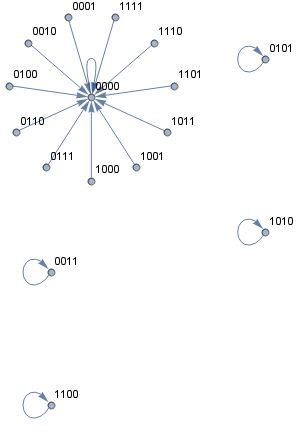
\includegraphics[width=12cm, height=10cm]{./img/tam-2-life.png}
 \caption{Árboles generados en una matriz de 2x2 con la regla de life}
 \label{fig:life2}
\end{center}
\end{figure}

\begin{figure}[H]
\begin{center}
 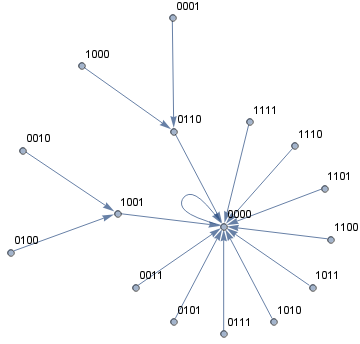
\includegraphics[width=12cm, height=8cm]{./img/tam-2-diffusion.png}
 \caption{Árboles generados en una matriz de 2x2 con la regla de difusión}
 \label{fig:difusion2}
\end{center}
\end{figure}

\begin{figure}[H]
\begin{center}
 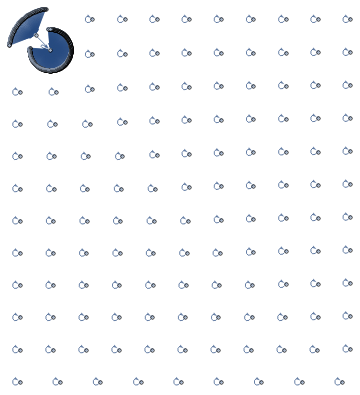
\includegraphics[width=12cm, height=10cm]{./img/tam-3-life.png}
 \caption{Árboles generados en una matriz de 3x3 con la regla de life}
 \label{fig:vida3}
\end{center}
\end{figure}

\begin{figure}[H]
\begin{center}
 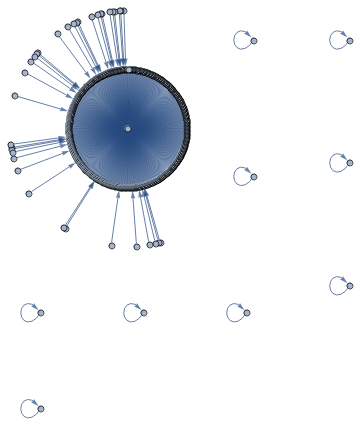
\includegraphics[width=12cm, height=10cm]{./img/tam-3-diffusion.png}
 \caption{Árboles generados en una matriz de 3x3 con la regla de difusión}
 \label{fig:difusion3}
\end{center}
\end{figure}

\subsection{Conclusiones}
A pesar de que solo se pudo observar el comportamiento en matrices de 2x2 y de 3x3 es fácil identificar el comportamiento característico de la regla de life y de la regla de difusión.

En difusión los árboles se encuentran más concentrados en menos grupos mientras que en life se generan muchos árboles lo cual es interesante considerando que en la regla de difusión la población tiende a crecer. Por lo que existe una relación en estas dos características.

Se podría decir que ya que de una configuración en especifica de la regla de difusión esta crece por lo que pasa por más configuraciones distintas que si se trabajara la misma configuración en life y es por esto que la cantidad de árboles es menor en la regla de difusión que en la de life.
